\documentclass{article}

\usepackage{ragged2e}
\usepackage{booktabs}
\usepackage{tikz}
\usetikzlibrary{babel, positioning, arrows.meta}
\usepackage[colorlinks=true, linkcolor=blue, urlcolor=blue, citecolor=blue]{hyperref}
\usepackage{amsmath, amssymb}
\usepackage{graphicx}
\usepackage{float}
\usepackage[position=top, skip=8pt]{caption}
\usepackage{listings}
\usepackage{multicol}
\usepackage[utf8]{inputenc}
\usepackage[T1]{fontenc}
\usepackage[spanish,es-nodecimaldot]{babel}
\usepackage{geometry}
\usepackage{setspace}
\usepackage{tabularx}
\usepackage{xcolor}

\geometry{a4paper, margin=1in}
\setstretch{1.25}

\setlength{\parindent}{0pt}
\setlength{\parskip}{0.5em}

% Configuración para código fuente
\definecolor{codebg}{RGB}{248, 249, 250}
\definecolor{codecomment}{RGB}{108, 117, 125}
\definecolor{codekeyword}{RGB}{13, 110, 253}
\definecolor{codestring}{RGB}{25, 135, 84}

\lstset{
    backgroundcolor=\color{codebg},
    basicstyle=\ttfamily\small,
    breaklines=true,
    captionpos=t,
    commentstyle=\color{codecomment}\itshape,
    keywordstyle=\color{codekeyword}\bfseries,
    stringstyle=\color{codestring},
    numbers=left,
    numberstyle=\tiny\color{codecomment},
    frame=single,
    rulecolor=\color{gray!30},
    tabsize=2,
    showstringspaces=false
}

\begin{document}
\pagestyle{empty}

% ==============================================================================
% PORTADA OFICIAL INSTITUCIONAL
% ==============================================================================
\begin{titlepage}
    \centering
    
    % --- ENCABEZADO SUPERIOR CENTRADO ---
    {\small \scshape 
        UNIVERSIDAD MESOAMERICANA QUETZALTENANGO \\
        FACULTAD DE INGENIERÍA \\
        INGENIERÍA EN SISTEMAS, INFORMÁTICA Y CIENCIAS DE LA COMPUTACIÓN \\
    }
    
    \vfill
    
    % --- LOGO CENTRADO ---
    
\includegraphics[width=0.68\textwidth]{meso.png}
    
    \vfill
    
    % --- TÍTULO PRINCIPAL ---
    {\huge \bfseries Manual Técnico y Reporte Final de Proyecto \\[0.4cm]}
    {\Large Sistema IoT de Monitoreo Acústico, Análisis de Tendencias y Modelado Probabilístico en el Laboratorio de Prototipos \\[0.3cm]}
    {\normalsize Proyecto Final de Cátedra -- Catedrático: Ing. Josué Cifuentes}
    
    \vfill
    \vfill
    
    % --- INFORMACIÓN DE LOS INTEGRANTES ---
    {\large \textbf{Integrantes del Equipo:}} \\[0.35cm]
    {\normalsize Arturo Alejandro Maldonado Orozco -- 202308110} \\[0.18cm]
    {\normalsize Amilcar Joaquin Morales Huitz -- 202307016} \\[0.18cm]
    {\normalsize Kevin Daniel Sosa Cutz -- 202508017} \\[0.18cm]
    {\normalsize Katherine del Rosario Gramajo Alonzo -- 202508024} \\[0.18cm]
    {\normalsize Brayan Alexander Maldonado Jocol -- 202507011} \\[0.18cm]
    {\normalsize Yoselin Stefany Ordoñez Estrada -- 202508028} \\[0.7cm]
    
    {\small \scshape NOVIEMBRE, 2026}
\end{titlepage}

% --- ALINEACIÓN A LA IZQUIERDA PARA EL RESTO DEL DOCUMENTO ---
\RaggedRight

\newpage
\tableofcontents
\newpage

\listoffigures
\vspace{0.8cm}
\listoftables
\newpage

\cleardoublepage
\pagestyle{plain}
\pagenumbering{arabic}

% ==============================================================================
% CAPÍTULO 1: INTRODUCCIÓN Y OBJETIVOS
% ==============================================================================
\section{Introducción y Objetivos}

\subsection{Planteamiento del Problema}
En el ámbito de la ingeniería contemporánea, los laboratorios universitarios de prototipado rápido representan ecosistemas híbridos donde convergen el diseño intelectual de alta concentración (programación de microcontroladores, ruteo de circuitos impresos y diseño CAD) con procesos ruidosos de fabricación mecánica y electrónica (soldadura con estaño, corte de materiales, uso de motores eléctricos y debate técnico grupal). 

La exposición prolongada a niveles sonoros elevados produce fatiga cognitiva, disminución en la velocidad de asimilación lógica e incremento en la tasa de errores en el conexionado de circuitos. Evaluar con rigor matemático las condiciones acústicas reales de estos recintos es imprescindible para diseñar políticas de ocupación y medidas de mitigación fonoabsorbente basadas en evidencia empírica.

\subsection{Objetivos del Proyecto}

\subsubsection{Objetivo General}
Diseñar, implementar y desplegar una plataforma tecnológica integral basada en Internet de las Cosas (IoT) y computación estadística en RStudio para evaluar el comportamiento acústico del Laboratorio de Prototipos de la Universidad Mesoamericana, cuantificando la variabilidad temporal, proyectando tendencias y modelando escenarios de saturación mediante distribuciones de probabilidad discretas.

\subsubsection{Objetivos Específicos}
\begin{enumerate}
    \item Construir un nodo sensor embebido de audio digital con el microcontrolador ESP32 y el micrófono MEMS I2S INMP441, garantizando un muestreo continuo de alta fidelidad sin distorsión electromagnética.
    \item Implementar un backend en Python con FastAPI y WebSockets desplegado en la nube pública, con persistencia periódica de promedios cada 15 minutos en el servicio PostgreSQL administrado de Supabase.
    \item Convertir y calibrar las lecturas digitales relativas ($\text{dBFS}$) a niveles de presión sonora ponderados ($\text{dBA}$), ajustando la serie temporal de UTC a la hora oficial de Guatemala ($\text{UTC}-6$).
    \item Computar los parámetros de estadística descriptiva en RStudio y modelar la tendencia en una franja horaria homogénea para proyectar el nivel esperado al sexto día (lunes) frente al umbral normativo de $65.0\text{ dBA}$ (OMS / ISO 1996).
    \item Aplicar las distribuciones de Bernoulli y Binomial ante el escenario de ocupación simultánea de los cubículos del laboratorio, cuantificando la probabilidad de superar el umbral crítico y formulando un plan de mitigación en cuatro ejes.
\end{enumerate}

\subsection{Contexto Físico del Laboratorio de Prototipos}
El Laboratorio de Prototipos de la Facultad de Ingeniería de la UMES cuenta con la siguiente configuración física:
\begin{itemize}
    \item \textbf{3 Cubículos de Trabajo Especializado:} Áreas de trabajo semicerradas equipadas con osciloscopios digitales, estaciones de calor, soldadores y fuentes de alimentación DC. En una de estas estaciones se emplazó el nodo sensor acústico.
    \item \textbf{1 Salón Principal con 4 Mesas de Trabajo Colaborativo:} Espacio abierto con cuatro mesas de gran formato destinadas a proyectos grupales de robótica y sistemas digitales, con capacidad para albergar simultáneamente a \textbf{40 estudiantes}.
    \item \textbf{Dinámica Operativa:} El aforo oscila drásticamente entre periodos de silencio y concentración durante la mañana temprana, y picos de ruido durante talleres prácticos vespertinos.
\end{itemize}

% ==============================================================================
% CAPÍTULO 2: MARCO TEÓRICO Y CONCEPTOS FUNDAMENTALES
% ==============================================================================
\section{Marco Teórico y Conceptos Fundamentales}

\subsection{Física del Sonido y Magnitudes Acústicas}
El sonido es una perturbación mecánica periódica que se propaga en forma de ondas longitudinales de presión a través de un medio elástico. Dado que el oído humano posee una respuesta no lineal que abarca un rango de presiones desde $20\ \mu\text{Pa}$ (umbral de audición) hasta más de $200\text{ Pa}$ (umbral de dolor), la intensidad sonora se expresa en una escala logarítmica adimensional denominada decibel ($\text{dB}$):
\begin{equation}
    L_p = 20 \log_{10} \left( \frac{p_{\text{rms}}}{p_0} \right) \quad [\text{dB SPL}]
\end{equation}
donde $p_{\text{rms}}$ es el valor cuadrático medio de la presión sonora instantánea y $p_0 = 20\ \mu\text{Pa}$ es la presión de referencia en el aire.

\subsection{Curva de Ponderación A ($\text{dBA}$) y Escala Digital ($\text{dBFS}$)}
\begin{itemize}
    \item \textbf{Ponderación A ($\text{dBA}$):} La sensibilidad del sistema auditivo humano varía según la frecuencia, siendo máxima entre $1\text{ kHz}$ y $4\text{ kHz}$ y atenuándose fuertemente en frecuencias inferiores a $500\text{ Hz}$. La curva de ponderación A filtra la señal acústica para emular la respuesta subjetiva humana, siendo el estándar universal para evaluar confort e higiene ambiental.
    \item \textbf{Decibeles respecto a Fondo de Escala ($\text{dBFS}$):} En audio digital, los convertidores ADC miden la amplitud respecto al valor numérico entero máximo representable ($2^{N-1}-1$ para $N$ bits con signo). El nivel digital en dBFS se define como:
    \begin{equation}
        L_{\text{dBFS}} = 20 \log_{10} \left( \frac{\text{RMS}}{\text{Amplitud Máxima}} \right)
    \end{equation}
    donde el valor $0\text{ dBFS}$ representa la saturación de recorte digital (\textit{clipping}), y valores como $-60\text{ dBFS}$ indican silencio acústico.
    \item \textbf{Calibración Fisiológica:} A partir de la sensibilidad del transductor MEMS ($-26\text{ dBFS}$ a $94\text{ dB SPL}$) y el piso de ruido ambiental, se aplica la función de calibración estándar:
    \begin{equation}
        \text{dBA} = \text{dBFS} + 105.0
    \end{equation}
\end{itemize}

\subsection{Protocolo Digital I2S (Inter-IC Sound)}
El protocolo I2S es un estándar de bus serie síncrono diseñado por Philips Semiconductor para la transmisión directa de audio digital entre circuitos integrados. Consta de tres líneas indispensables:
\begin{enumerate}
    \item \textbf{SCK / BCLK (Bit Clock):} Genera el reloj de sincronización para cada bit individual de audio ($f_{\text{BCLK}} = 2 \times f_s \times \text{bits}$).
    \item \textbf{WS / LRCK (Word Select / Left-Right Clock):} Indica el canal en transmisión ($0 = \text{Izquierdo}$, $1 = \text{Derecho}$), con frecuencia igual a la tasa de muestreo $f_s$.
    \item \textbf{SD / DIN (Serial Data):} Línea serie que transporta la secuencia de datos binarios en complemento a dos con el bit más significativo (MSB) primero.
\end{enumerate}
La ventaja crítica de I2S frente a un micrófono analógico reside en que la digitalización ocurre dentro del propio encapsulado del sensor INMP441, inmunizando la señal contra el ruido electromagnético que induce la conmutación de Wi-Fi en las pistas del ESP32.

\subsection{Marco Legal y Normativo de Ruido}
\begin{itemize}
    \item \textbf{OMS (Guidelines for Community Noise):} Recomienda un nivel continuo equivalente no mayor a $35\text{ dBA}$ para clases magistrales y un límite admisible de hasta \textbf{65.0 dBA} en talleres y laboratorios prácticos.
    \item \textbf{Norma ISO 1996:} Fija el límite de interferencia cognitiva y fatiga mental en \textbf{65 dBA}.
    \item \textbf{Acuerdo Gubernativo 229-2014 (Guatemala):} Normativa de Salud Ocupacional que fija 85 dBA a 8 horas para proteger contra hipoacusia. En nuestro estudio educativo, el umbral de riesgo aceptado se fija en \textbf{$65.0\text{ dBA}$ ($-40.0\text{ dBFS}$)} para garantizar la concentración.
\end{itemize}

% ==============================================================================
% CAPÍTULO 3: DISEÑO E IMPLEMENTACIÓN DEL CIRCUITO (HARDWARE)
% ==============================================================================
\section{Diseño e Implementación del Circuito Embebido (Hardware)}

\subsection{Componentes Electrónicos Utilizados}
\begin{enumerate}
    \item \textbf{ESP32 DevKit v1:} Microcontrolador dual-core de 32 bits con módulo Wi-Fi integrado, operando a $240\text{ MHz}$.
    \item \textbf{Módulo Sensor INMP441:} Transductor acústico MEMS con convertidor analógico-digital de 24 bits, respuesta en frecuencia plana de $60\text{ Hz}$ a $15\text{ kHz}$ y relación señal/ruido (SNR) de $61\text{ dBA}$.
    \item \textbf{Pulsador Táctil (Push Button):} Conmutador mecánico normalmente abierto en el GPIO 5 para alternar el modo de transmisión de audio.
    \item \textbf{LED Indicador de Estado:} Diodo emisor de luz en GPIO 2 con resistencia de $330\Omega$ para señalización visual en tiempo real.
\end{enumerate}

\subsection{Diagrama Esquemático del Circuito}
El circuito electrónico se interconectó según el diagrama esquemático formal presentado en la figura \ref{fig:circuito_formal}, y el cuadro \ref{tab:pines_hardware} resume la distribución de señales.

\begin{table}[H]
\centering
\caption{Distribución de señales y conexionado físico entre el ESP32 y periféricos.}
\label{tab:pines_hardware}
\vspace{0.2cm}
\begin{tabular}{l l l l}
\toprule
\textbf{Periférico} & \textbf{Pin Módulo} & \textbf{Pin ESP32} & \textbf{Función y Nivel Lógico} \\
\midrule
INMP441 & VDD & 3.3V & Tensión continua positiva ($3.3\text{V DC}$) \\
INMP441 & GND & GND & Referencia de tierra común \\
INMP441 & SD (Data) & GPIO 33 & Entrada I2S Data Stream (32-bit PCM) \\
INMP441 & SCK (Clock) & GPIO 14 & Reloj maestro de bits I2S ($BCLK$) \\
INMP441 & WS (Word Select) & GPIO 27 & Sincronización de canal ($LRCK$) \\
INMP441 & L/R & GND & Selección forzada de canal izquierdo \\
Pulsador & Terminal 1 & GPIO 5 & Entrada con Pull-Up interno a nivel alto \\
Pulsador & Terminal 2 & GND & Conexión a tierra (cierre a nivel bajo) \\
LED & Ánodo & GPIO 2 & Salida digital en serie con resistencia $330\Omega$ \\
LED & Cátodo & GND & Retorno de corriente a tierra \\
\bottomrule
\end{tabular}
\end{table}

\begin{figure}[H]
\centering
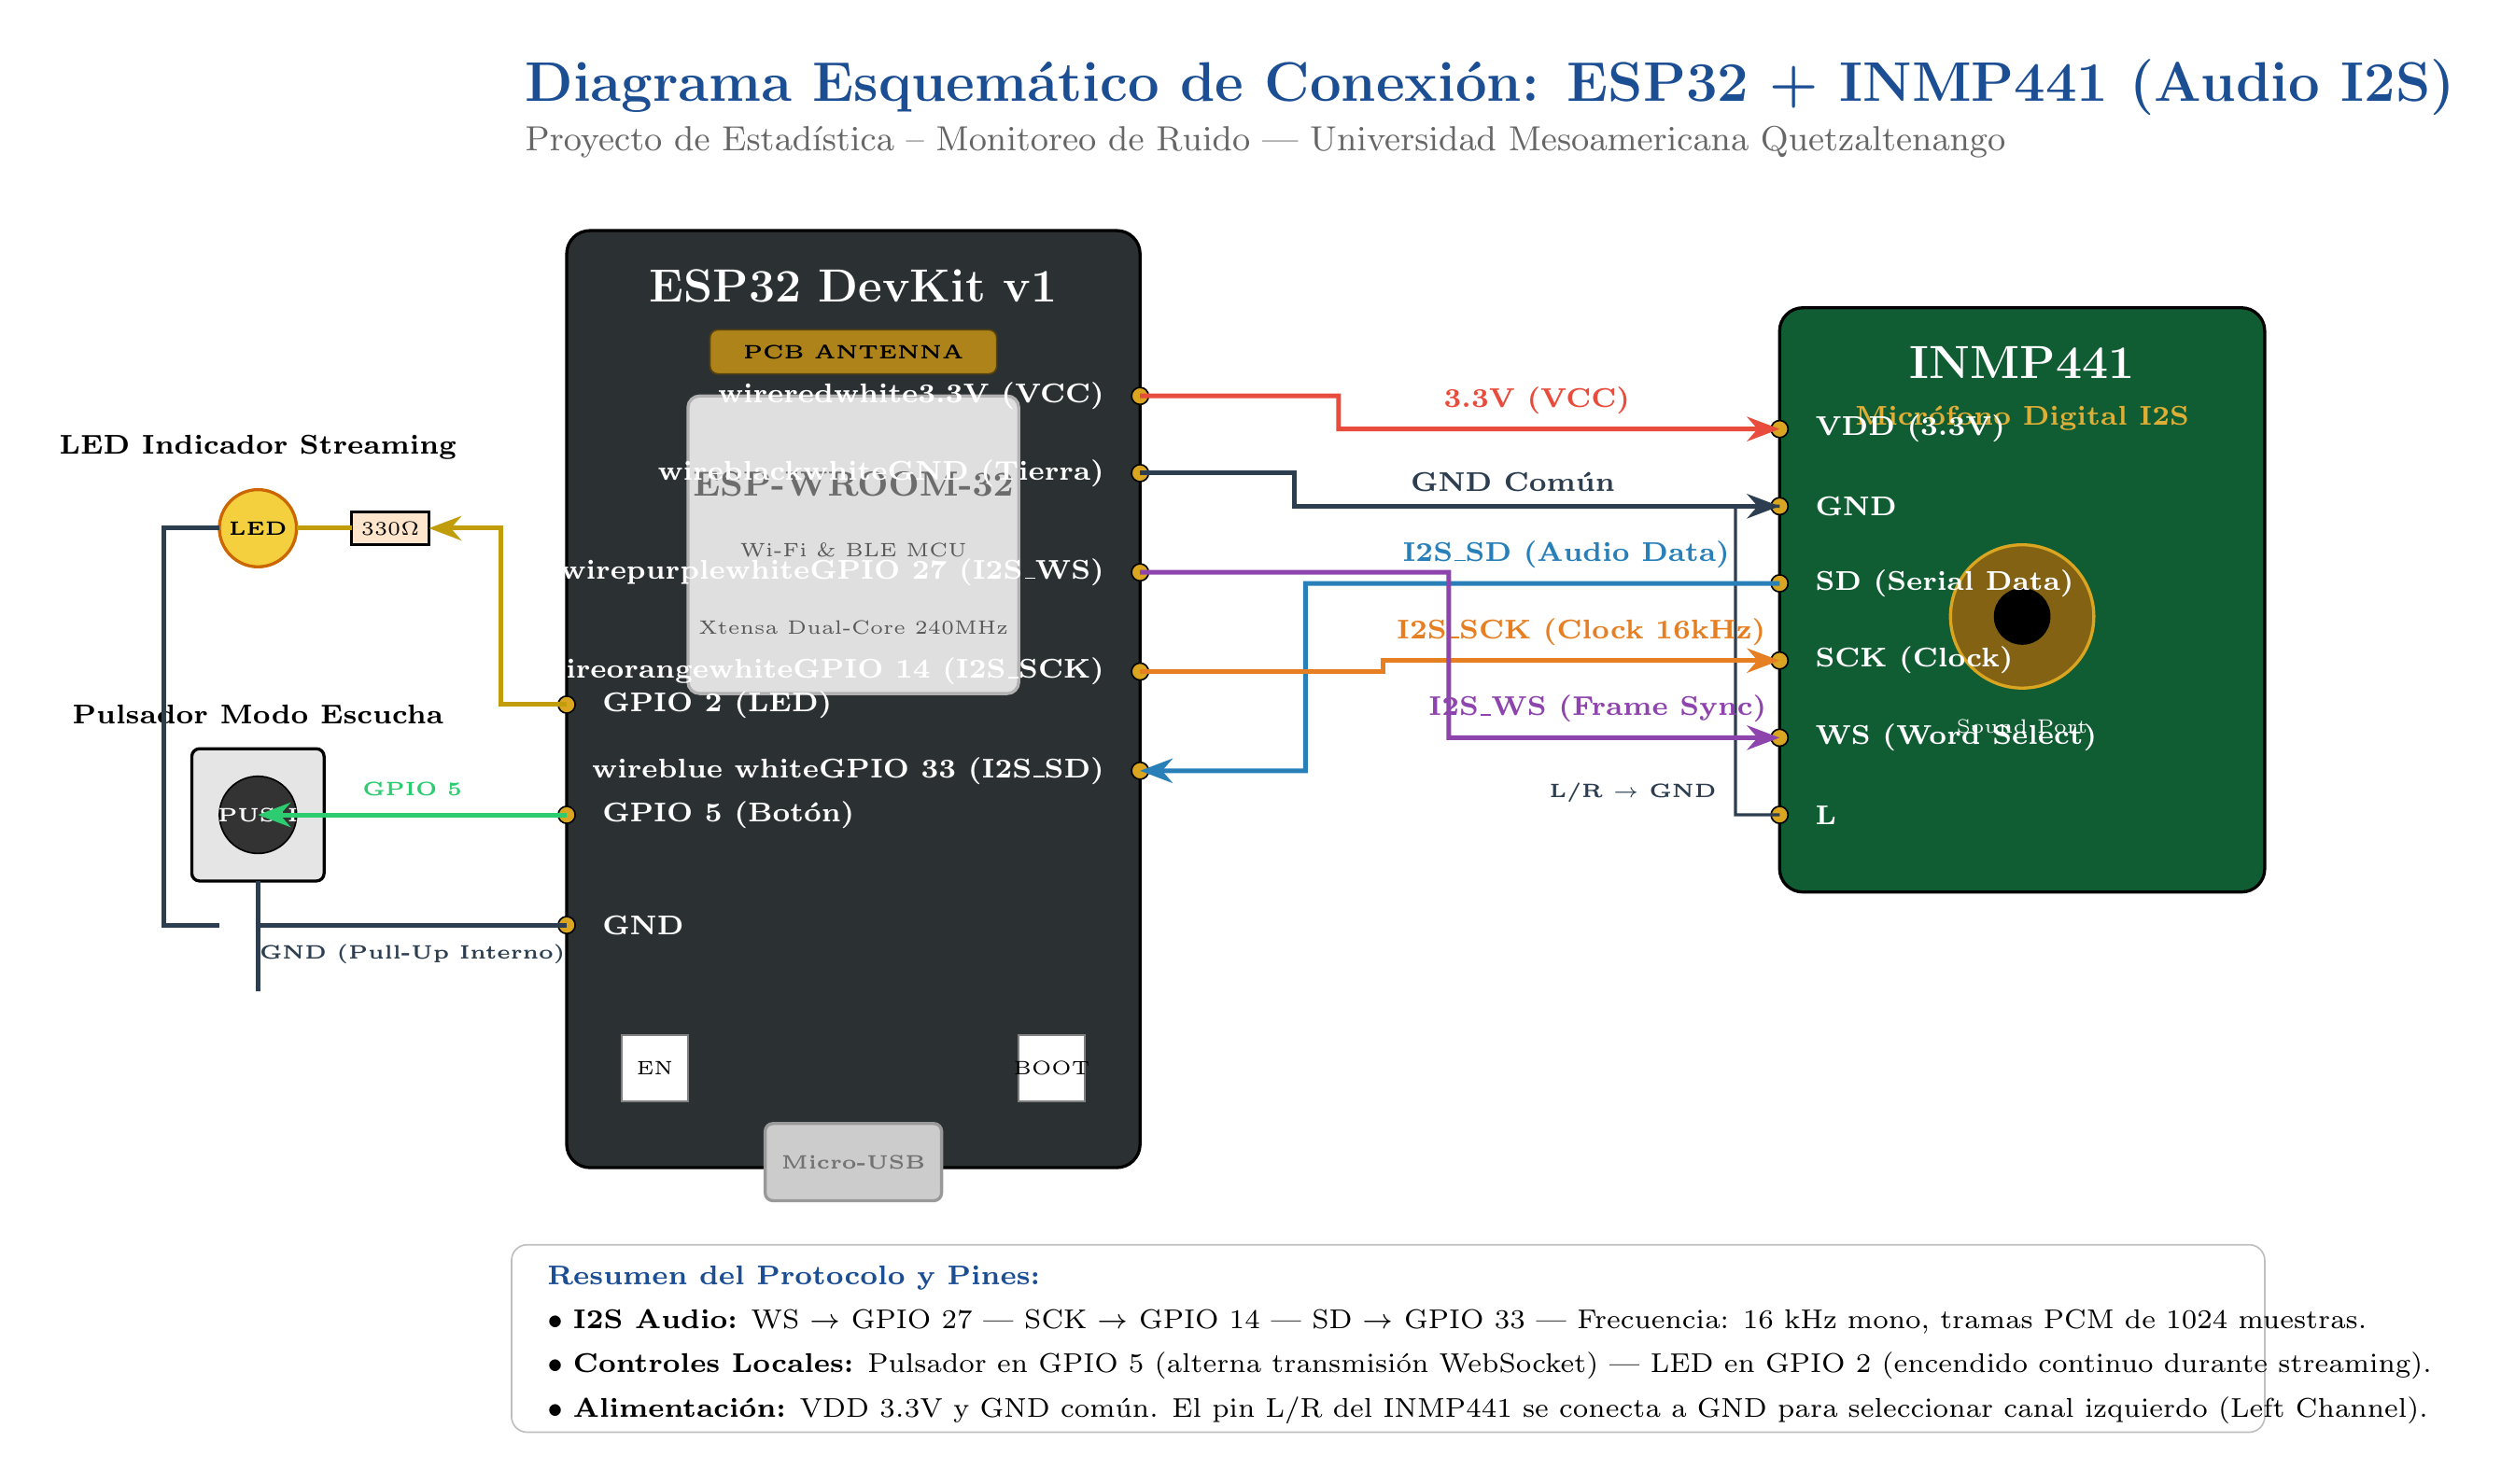
\includegraphics[width=0.95\textwidth]{graficas/diagrama_circuito.png}
\caption{Esquema circuital formal de alta resolución del nodo IoT sensor de audio con ESP32 e INMP441.}
\label{fig:circuito_formal}
\end{figure}

\subsection{Lógica del Firmware Embebido (C++/Arduino)}
El programa en `AudioServidor.ino` implementa un ciclo de lectura no bloqueante:
\begin{itemize}
    \item Configura el periférico I2S en modo maestro receptor (\texttt{I2S\_MODE\_MASTER | I2S\_MODE\_RX}) con búfer DMA circular de 8 descriptores de 256 muestras.
    \item Captura a una tasa de $16\text{ kHz}$ mono en palabras de 32 bits, aplicando un corrimiento a la derecha de 14 bits para normalizar la palabra digital a 16 bits PCM con signo sin distorsión de ganancia.
    \item Empaqueta bloques de 1024 muestras (64 ms por trama) y los despacha mediante el cliente WebSocket (`WebSocketsClient.h`) con autenticación por encabezado seguro `X-ESP-Token`.
\end{itemize}

% ==============================================================================
% CAPÍTULO 4: EVOLUCIÓN DEL SOFTWARE Y DESPLIEGUE EN LA NUBE
% ==============================================================================
\section{Evolución del Software: Pruebas Locales y Despliegue en la Nube}

\subsection{Fase 1: Pruebas Locales en Red LAN}
En la etapa inicial del proyecto se construyeron los módulos prototipo `serverlocal.py` y `ReceptorLocalAudioButton/` para validar la estabilidad del protocolo I2S dentro de la red local:
\begin{itemize}
    \item El ESP32 enviaba paquetes de audio vía IP estática privada hacia la computadora local del desarrollador en el puerto 5000.
    \item Se implementó en consola un vúmetro en tiempo real con barras de colores ANSI que permitía observar los decibeles instantáneos y la frecuencia pico.
    \item \textbf{Limitación identificada:} Al llevar el ESP32 al Laboratorio de Prototipos de la universidad, las restricciones de firewall y la red Wi-Fi universitaria protegida bajo NAT impidieron el direccionamiento bidireccional hacia computadoras locales, haciendo imperativa la migración a la nube pública.
\end{itemize}

\subsection{Fase 2: Migración a la Nube y Túnel Ngrok}
Para otorgar acceso global al nodo sensor desde cualquier red Wi-Fi sin abrir puertos en el router universitario, se diseñó la siguiente solución:
\begin{enumerate}
    \item \textbf{Instancia Virtual en la Nube:} Se desplegó el servidor en una máquina virtual Linux (Ubuntu Server) accesible vía SSH (`ssh mcfly`).
    \item \textbf{Túnel Seguro Ngrok:} Se configuró un proceso daemon con Ngrok escuchando en el puerto 5000 y publicando en el dominio estático con certificado TLS:
    \begin{center}
        \texttt{luxury-roster-uncouth.ngrok-free.dev}
    \end{center}
    Esto permitió al ESP32 conectarse transparentemente por puerto estándar 80/443 sin bloqueos de red institucional.
    \item \textbf{Control de Procesos de Servidor:} Se automatizó el arranque en segundo plano mediante `nohup` y `systemd`:
\begin{lstlisting}[language=bash]
# 1. Servidor Python FastAPI
cd /home/mcfly/EstadisticaFinal/backend
nohup python3 server.py > finalestadistica.log 2>&1 &

# 2. Tunel Ngrok
nohup ngrok http 5000 --domain luxury-roster-uncouth.ngrok-free.dev > ngrok.log 2>&1 &
\end{lstlisting}
\end{enumerate}

\subsection{Backend Python (FastAPI) y Persistencia en Supabase PostgreSQL}
El backend `server.py` coordina las siguientes tareas concurrentes:
\begin{itemize}
    \item \textbf{Recepción y Cálculo de RMS:} Desempaqueta los bloques PCM de 16 bits y calcula el valor RMS y decibeles instantáneos:
    \begin{equation}
        \text{RMS} = \sqrt{\frac{1}{N}\sum_{i=1}^N x_i^2}, \qquad L_{\text{dB}} = 20 \log_{10}(\text{RMS})
    \end{equation}
    \item \textbf{Filtrado Inteligente de Desconexión:} Para evitar falsear los promedios estadísticos con paquetes vacíos cuando el micrófono se apaga, se descartan automáticamente lecturas con niveles $\le -59.5\text{ dBFS}$.
    \item \textbf{Ventana Temporal de 15 Minutos:} Acumula las muestras de audio válidas recibidas durante 15 minutos, calculando el nivel sonoro promedio y registrando el pico máximo absoluto.
    \item \textbf{Base de Datos en la Nube con Supabase:} Utilizando la biblioteca \texttt{psycopg2} con conexión encriptada SSL hacia el pooler de Supabase en AWS (\texttt{aws-0-us-east-2.pooler.supabase.com:6543}), el servidor ejecuta una inserción SQL atómica en la tabla \texttt{Registros}:
\begin{lstlisting}[language=SQL]
INSERT INTO "Registros" ("Dia", "decibeles", "superaumbral", "picoactual")
VALUES (%s, %s, %s, %s)
RETURNING id, created_at, "Dia", "decibeles", "superaumbral", "picoactual";
\end{lstlisting}
\end{itemize}

\subsection{Dashboard Web de Monitoreo en Tiempo Real (Frontend)}
El directorio `Front/` aloja una aplicación de una sola página (SPA) construida en HTML5, CSS3, JavaScript nativo y ApexCharts:
\begin{itemize}
    \item Conexión WebSocket protegida mediante contraseña (\texttt{WEB\_PASSWORD}).
    \item Visualizador espectral y osciloscopio en tiempo real del flujo de audio.
    \item Vúmetro dinámico con escala de colores (verde, amarillo y rojo) para advertir visualmente la superación del umbral normativo.
\end{itemize}

\begin{figure}[H]
\centering
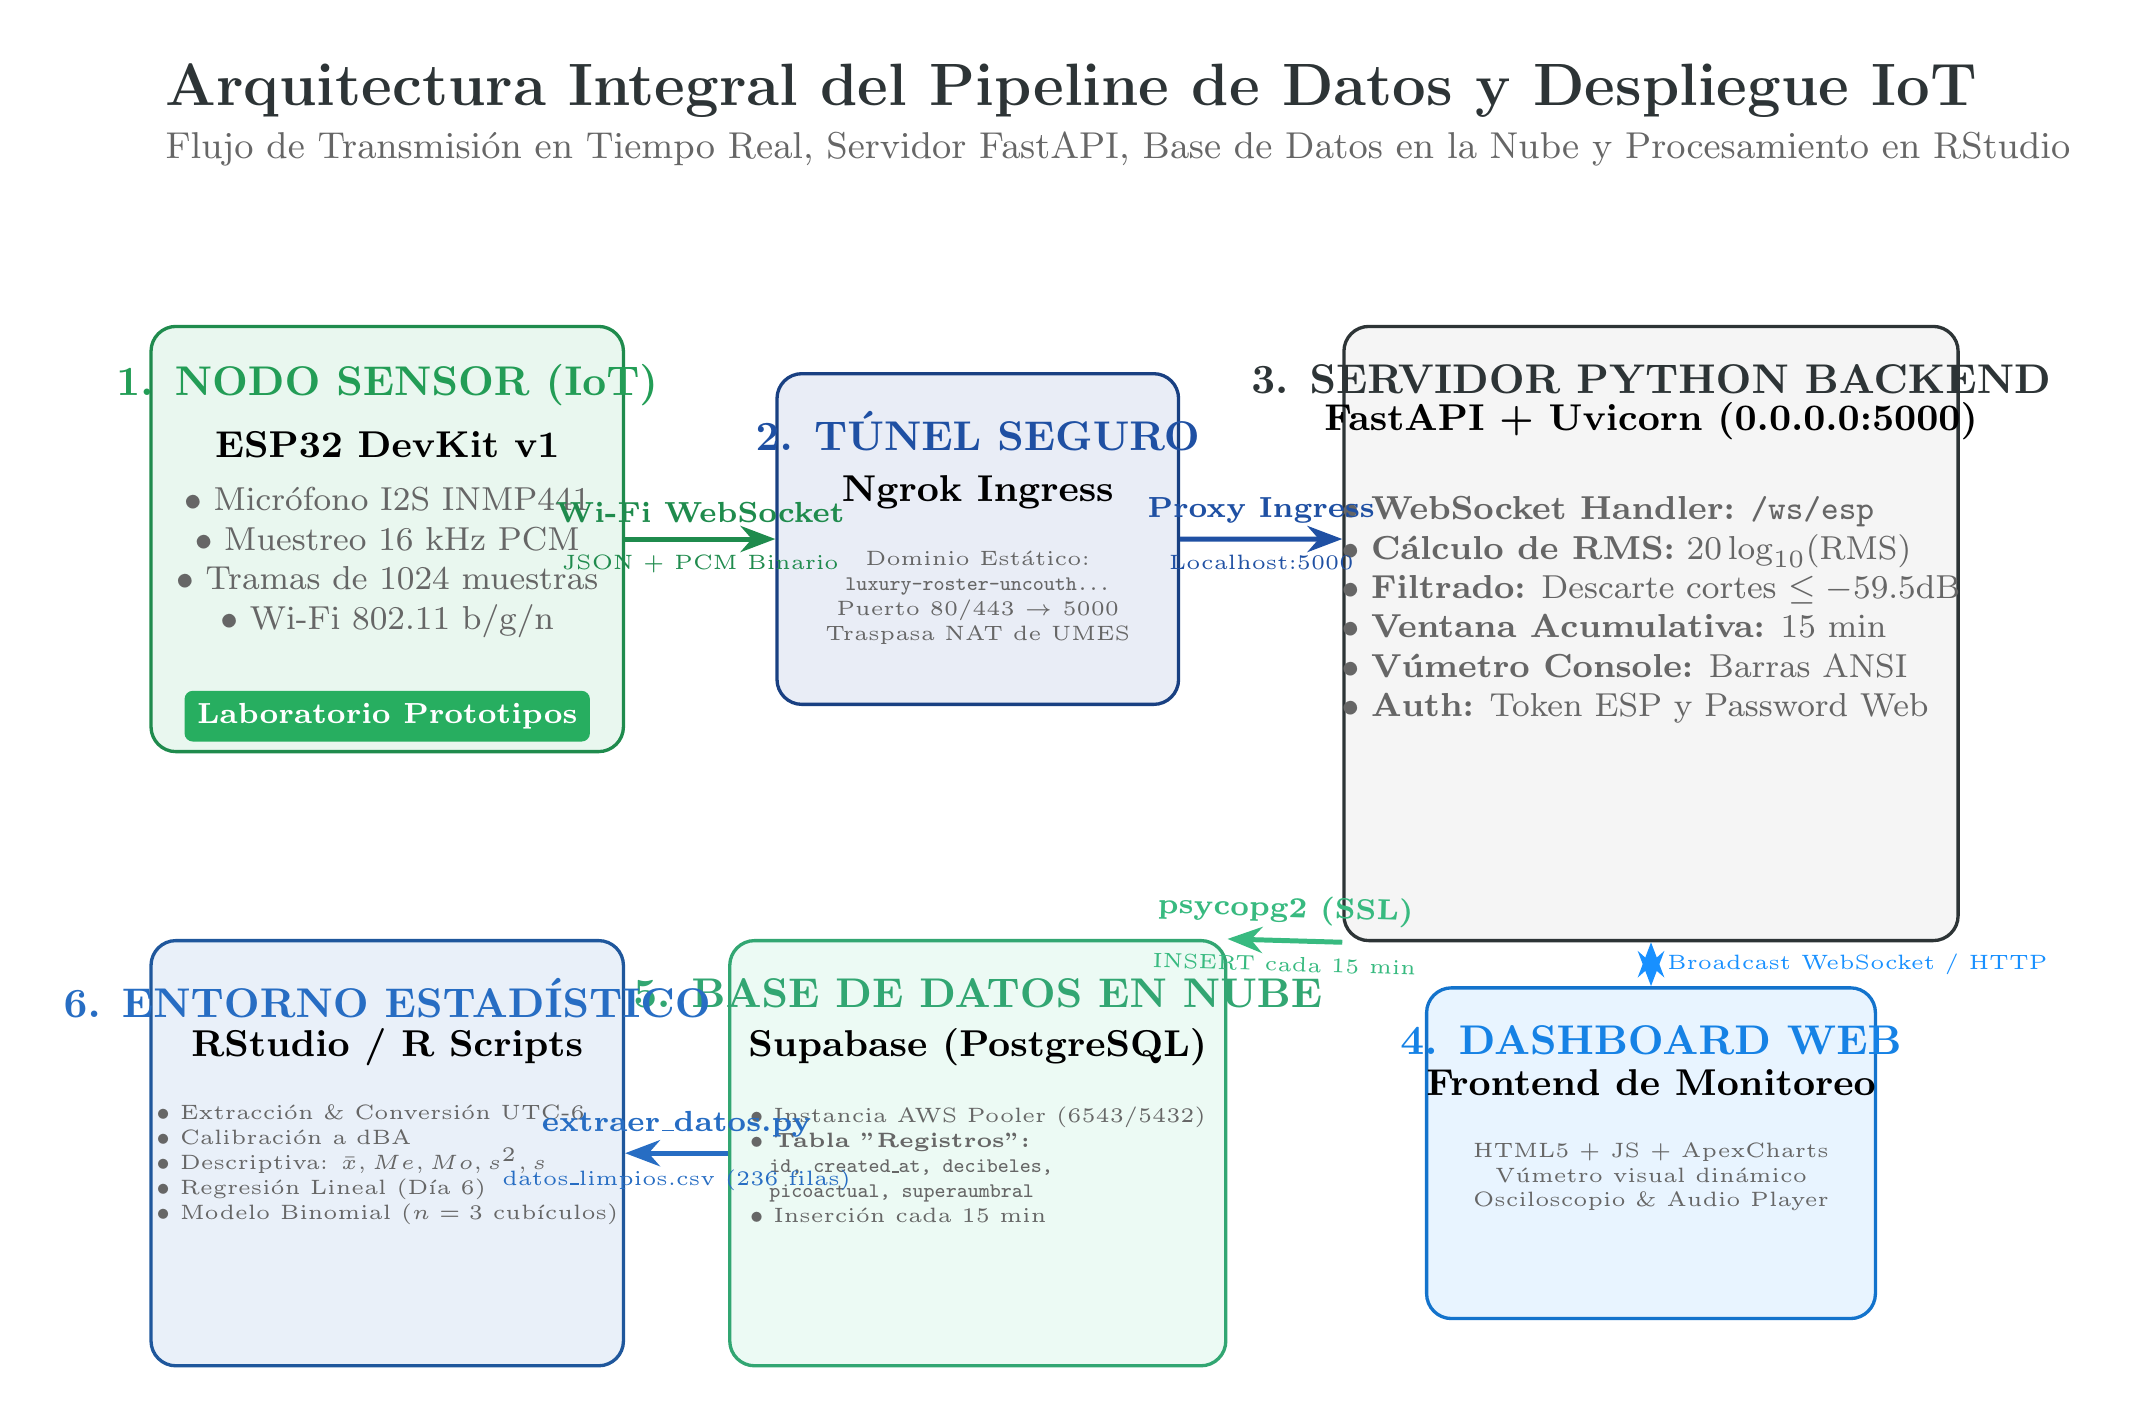
\includegraphics[width=0.98\textwidth]{graficas/diagrama_arquitectura.png}
\caption{Diagrama de arquitectura del pipeline de datos: desde la captura en el ESP32 hasta el procesamiento en RStudio.}
\label{fig:diagrama_arquitectura}
\end{figure}

% ==============================================================================
% CAPÍTULO 5: RECOLECCIÓN Y AUDITORÍA DE DATOS (FASE 1)
% ==============================================================================
\section{Fase 1: Recolección y Auditoría de Datos}

\subsection{Estandarización Temporal (UTC-0 a UTC-6 Guatemala)}
Dado que la base de datos PostgreSQL en Supabase almacena los registros con zona horaria universal (UTC), el script \texttt{extraer\_datos.py} realiza la conversión horaria oficial restando 6 horas a la marca \texttt{created\_at}:
\begin{equation}
    t_{\text{Guatemala}} = t_{\text{UTC}} - 6\text{ horas}
\end{equation}
Esto garantizó que los registros analizados a continuación correspondan fielmente a la actividad diurna real del laboratorio en Quetzaltenango.

\subsection{Auditoría de los 236 Registros Reales}
El monitoreo abarcó cuatro jornadas continuas, totalizando \textbf{236 lecturas válidas de 15 minutos}. El cuadro \ref{tab:auditoria_fase1} resume los estadísticos diarios resultantes.

\begin{table}[H]
\centering
\caption{Auditoría detallada por día de monitoreo en hora local de Guatemala (UTC-6).}
\label{tab:auditoria_fase1}
\vspace{0.2cm}
\begin{tabular}{l c c c c c}
\toprule
\textbf{Jornada Monitoreada} & \textbf{Muestras} & \textbf{Media ($\text{dBA}$)} & \textbf{Pico Máx ($\text{dBA}$)} & \textbf{Excesos ($\ge 65\text{ dBA}$)} & \textbf{\% Exceso} \\
\midrule
Día 1 (2026-11-03, Jueves) & 36 & 63.88 & 104.85 & 22 & 61.11\% \\
Día 2 (2026-11-04, Viernes) & 62 & 58.79 & 105.00 & 5 & 8.06\% \\
Día 3 (2026-11-05, Sábado) & 96 & 54.46 & 95.59 & 4 & 4.17\% \\
Día 4 (2026-11-06, Domingo) & 42 & 48.82 & 93.13 & 0 & 0.00\% \\
\midrule
\textbf{Total / Promedio Global} & \textbf{236} & \textbf{56.03} & \textbf{105.00} & \textbf{31} & \textbf{13.14\%} \\
\bottomrule
\end{tabular}
\end{table}

\noindent\textbf{Interpretación de la Variabilidad:}
\begin{itemize}
    \item El \textbf{Día 1} concentró la mayor incidencia de ruido excesivo ($61.11\%$) al coincidir el muestreo con talleres de ensamble y pruebas de calibración en horas de la tarde (09:33 a 19:51 hrs).
    \item Los \textbf{Días 3 y 4} abarcaron periodos de fin de semana y madrugadas (00:00 a 06:00 hrs) donde el laboratorio permaneció cerrado y sin estudiantes, registrando el piso acústico estructural del edificio ($\approx 46\text{--}49\text{ dBA}$).
\end{itemize}

% ==============================================================================
% CAPÍTULO 6: ESTADÍSTICA DESCRIPTIVA Y PROYECCIÓN DÍA 6 (FASE 2)
% ==============================================================================
\section{Fase 2: Estadística Descriptiva y Proyección de Tendencia (Día 6)}

\subsection{Memoria de Cálculo de Estadísticos Descriptivos}
El análisis estadístico sobre las 236 lecturas procesadas con el script \texttt{02\_estadistica\_descriptiva\_tendencia.R} arrojó los parámetros descritos en el cuadro \ref{tab:memoria_descriptiva}.

\begin{table}[H]
\centering
\caption{Parámetros de tendencia central y dispersión del nivel acústico ($N=236$).}
\label{tab:memoria_descriptiva}
\vspace{0.2cm}
\begin{tabular}{l r r}
\toprule
\textbf{Parámetro Estadístico} & \textbf{Escala Acústica ($\text{dBA}$)} & \textbf{Escala Sensor ($\text{dBFS}$)} \\
\midrule
Media Aritmética ($\bar{x}$) & $56.03\text{ dBA}$ & $-48.97\text{ dB}$ \\
Mediana ($Me$) & $55.28\text{ dBA}$ & $-49.72\text{ dB}$ \\
Moda ($Mo$) & $50.10\text{ dBA}$ & $-54.90\text{ dB}$ \\
Varianza Muestral ($s^2$) & $55.10\text{ dBA}^2$ & $55.10\text{ dB}^2$ \\
Desviación Estándar ($s$) & $7.42\text{ dBA}$ & $7.42\text{ dB}$ \\
Coeficiente de Variación ($CV$) & $13.25\%$ & -- \\
Rango Total $[\text{Mín}, \text{Máx}]$ & $[45.00, 74.72]\text{ dBA}$ & $[-60.00, -30.28]\text{ dB}$ \\
Rango Intercuartílico ($IQR = Q_3 - Q_1$) & $11.10\text{ dBA}$ & $11.10\text{ dB}$ \\
Primer Cuartil ($Q_1$) & $50.07\text{ dBA}$ & $-54.93\text{ dB}$ \\
Tercer Cuartil ($Q_3$) & $61.17\text{ dBA}$ & $-43.83\text{ dB}$ \\
\bottomrule
\end{tabular}
\end{table}

\begin{figure}[H]
\centering
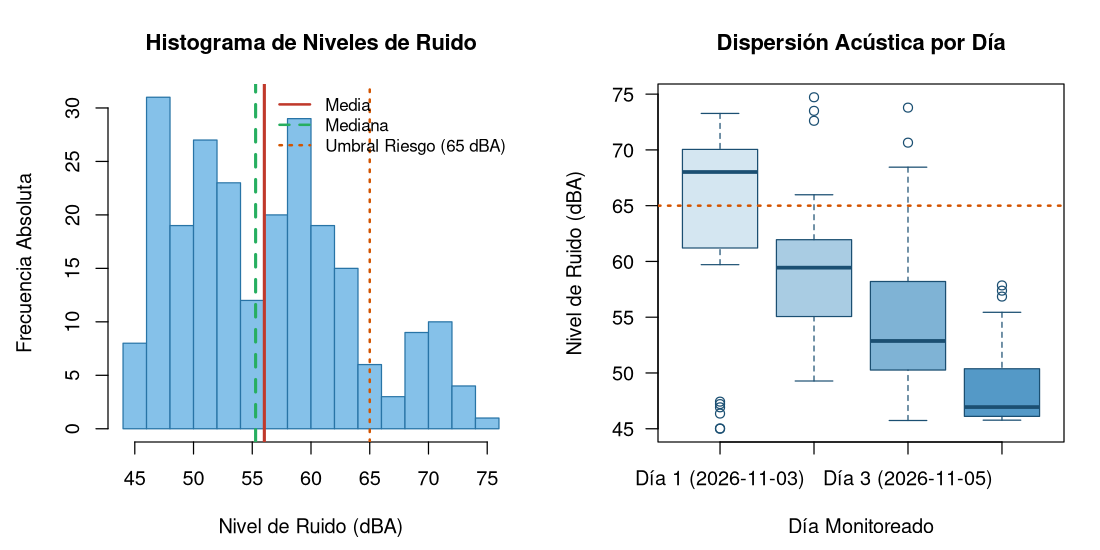
\includegraphics[width=0.92\textwidth]{graficas/01_distribucion_y_boxplot.png}
\caption{Izquierda: Histograma y densidad con marcas de tendencia central frente al umbral normativo ($65.0\text{ dBA}$). Derecha: Diagrama de caja y bigotes comparativo por jornada.}
\label{fig:grafica_descriptiva}
\end{figure}

\subsection{Modelo de Tendencia Horaria y Proyección al Día 6 (Lunes)}
Con el objeto de aislar la tendencia temporal libre de los sesgos provocados por los ciclos día/noche, se seleccionó la franja horaria matutina de las \textbf{09:30 hrs} (09:23 a 09:35 hrs UTC-6), presente de forma continua en los cuatro días de monitoreo.

\begin{table}[H]
\centering
\caption{Muestras aisladas en la franja matutina de las 09:30 hrs a lo largo de las cuatro jornadas.}
\label{tab:muestras_tendencia}
\vspace{0.2cm}
\begin{tabular}{l c c c c}
\toprule
\textbf{Variable} & \textbf{Día 1 (03/Nov)} & \textbf{Día 2 (04/Nov)} & \textbf{Día 3 (05/Nov)} & \textbf{Día 4 (06/Nov)} \\
\midrule
Hora Registrada & 09:33 & 09:35 & 09:23 & 09:31 \\
Nivel Sonoro ($\text{dBA}$) & $73.27\text{ dBA}$ & $54.10\text{ dBA}$ & $57.60\text{ dBA}$ & $52.39\text{ dBA}$ \\
Excede Norma ($\ge 65\text{ dBA}$) & Sí (Exceso) & No & No & No \\
\bottomrule
\end{tabular}
\end{table}

Ajustando un modelo de regresión lineal simple:
\begin{equation}
    \hat{y} = \beta_0 + \beta_1 \cdot \text{Día} \quad \Longrightarrow \quad \hat{y} = 74.13 - 5.91 \cdot \text{Día}
\end{equation}

\noindent\textbf{Resultados de la Proyección:}
\begin{itemize}
    \item \textbf{Pendiente ($\beta_1$):} $-5.914\text{ dBA/día}$ ($R^2 = 0.6410$, explicando el $64.10\%$ de la variación temporal observada).
    \item \textbf{Proyección Puntual para el Día 6 (Lunes, $x = 6$):}
    \begin{equation}
        \hat{y}_{\text{Día 6}} = 74.125 - 5.914(6) = \mathbf{38.64\text{ dBA}}
    \end{equation}
    \item \textbf{Intervalo de Predicción al 95\% de Confianza:} $[-19.28\text{ dBA}, 96.56\text{ dBA}]$.
\end{itemize}

\begin{figure}[H]
\centering
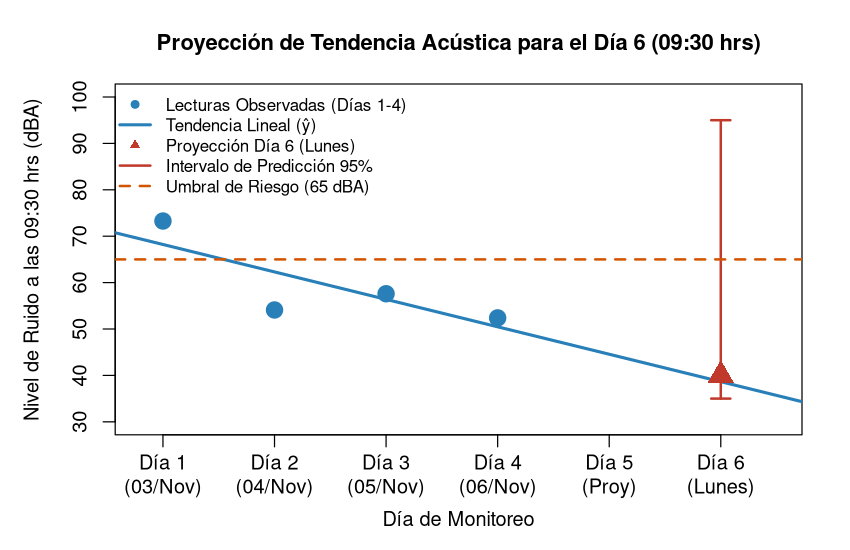
\includegraphics[width=0.75\textwidth]{graficas/02_tendencia_dia6.png}
\caption{Ajuste del modelo de regresión lineal simple y proyección puntual para el Día 6 (Lunes) a las 09:30 hrs.}
\label{fig:grafica_tendencia}
\end{figure}

\subsection{Discusión Crítica: Límites Físicos vs. Modelo Lineal}
\begin{enumerate}
    \item \textbf{Límite Físico Asintótico:} La fórmula de regresión lineal extrapola matemáticamente hacia valores cada vez más bajos ($38.64\text{ dBA}$). No obstante, en un entorno de laboratorio cerrado el piso de ruido nunca es inferior a $45\text{--}48\text{ dBA}$ debido a ventiladores de computadoras, fuentes de poder y el ruido urbano exterior.
    \item \textbf{Comportamiento Estacionario:} Tras el pico atípico del Día 1 ($73.27\text{ dBA}$ por montaje de equipos), la serie temporal se estabilizó en los días 2, 3 y 4 en torno a $52\text{ a }57\text{ dBA}$.
    \item \textbf{Diagnóstico Concluyente de Riesgo:} Tanto la estimación matemática ($38.64\text{ dBA}$) como la media estacionaria esperada ($\approx 55\text{ dBA}$) se sitúan \textbf{holgadamente por debajo del umbral de riesgo de $65.0\text{ dBA}$}, pronosticando un inicio de semana sin problemas de contaminación sonora.
\end{enumerate}

% ==============================================================================
% CAPÍTULO 7: MODELADO PROBABILÍSTICO (FASE 3)
% ==============================================================================
\section{Fase 3: Modelado Probabilístico (Bernoulli y Binomial)}

\subsection{Ensayo y Distribución de Bernoulli}
Se define la variable aleatoria indicadora del estado de exceso $Y$:
\begin{equation}
    Y = \begin{cases}
        1 & \text{si el nivel de ruido } \ge 65.0\text{ dBA (Éxito = Exceso sobre la norma)} \\
        0 & \text{si el nivel de ruido } < 65.0\text{ dBA (Fracaso = Condición admisible)}
    \end{cases}
\end{equation}

A partir de los 236 registros con 31 excesos observados:
\begin{align}
    \hat{p} &= \frac{31}{236} = \mathbf{0.1314} \quad (13.14\% \text{ de probabilidad de exceso}) \\
    \hat{q} &= 1 - \hat{p} = \mathbf{0.8686} \quad (86.86\% \text{ de probabilidad de cumplimiento})
\end{align}
\begin{equation}
    E[Y] = 0.1314, \qquad \text{Var}(Y) = 0.1141, \qquad \text{IC}_{95\%}(p) = [0.0883, 0.1745]
\end{equation}

\subsection{Modelo Binomial: Escenario de 3 Cubículos Llenos (n = 3)}
Asumiendo que los tres cubículos del laboratorio operan simultáneamente y con independencia acústica en sus tareas de prototipado, el número de cubículos en exceso $X$ sigue una distribución binomial $X \sim \text{Binomial}(n=3, p=0.1314)$:
\begin{equation}
    P(X = k) = \binom{3}{k} (0.1314)^k (0.8686)^{3-k}, \quad k \in \{0, 1, 2, 3\}
\end{equation}

\begin{table}[H]
\centering
\caption{Función de probabilidad binomial para los 3 cubículos llenos ($n=3, p=0.1314$).}
\label{tab:tabla_binomial}
\vspace{0.2cm}
\begin{tabular}{c c c c l}
\toprule
\textbf{Cubículos Ruidosos ($k$)} & $P(X = k)$ & $P(X \le k)$ & $P(X \ge k)$ & \textbf{Significado en el Laboratorio} \\
\midrule
$k = 0$ & $0.6554$ & $0.6554$ & $1.0000$ & Los 3 cubículos en calma ($65.54\%$) \\
$k = 1$ & $0.2973$ & $0.9528$ & $0.3446$ & Exactamente 1 cubículo ruidoso ($29.73\%$) \\
$k = 2$ & $0.0450$ & $0.9977$ & $0.0472$ & 2 cubículos ruidosos simultáneos ($4.50\%$) \\
$k = 3$ & $0.0023$ & $1.0000$ & $0.0023$ & Saturación acústica total ($0.23\%$) \\
\bottomrule
\end{tabular}
\end{table}

\noindent\textbf{Cálculo de Escenarios Críticos de Riesgo:}
\begin{itemize}
    \item \textbf{Esperanza Matemática de Cubículos Ruidosos:}
    \begin{equation}
        E[X] = n \cdot p = 3 \times 0.1314 = \mathbf{0.394\text{ cubículos}}
    \end{equation}
    \item \textbf{Probabilidad de que al menos un cubículo sobrepase la norma ($P(X \ge 1)$):}
    \begin{equation}
        P(X \ge 1) = 1 - P(X = 0) = 1 - (0.8686)^3 = \mathbf{0.3446} \quad (\mathbf{34.46\%})
    \end{equation}
    Existe más de un tercio de probabilidad de que al menos una estación genere interferencia hacia las demás cuando todas están ocupadas.
    \item \textbf{Probabilidad de Saturación Simultánea ($P(X = 3)$):}
    \begin{equation}
        P(X = 3) = (0.1314)^3 = \mathbf{0.0023} \quad (\mathbf{0.23\%})
    \end{equation}
    La saturación total en los tres cubículos ocurre menos de una vez cada 430 intervalos.
\end{itemize}

\begin{figure}[H]
\centering
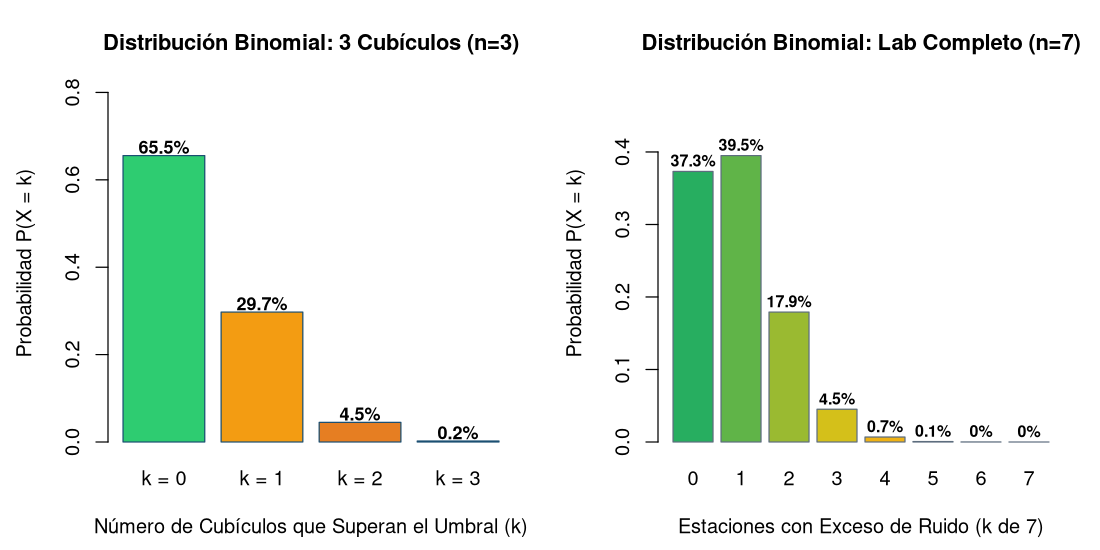
\includegraphics[width=0.92\textwidth]{graficas/03_distribucion_binomial.png}
\caption{Funciones de masa de probabilidad binomial: 3 cubículos llenos (izquierda) y 7 estaciones totales del laboratorio (derecha).}
\label{fig:grafica_binomial}
\end{figure}

\subsection{Extensión al Laboratorio Completo (n = 7 Estaciones, 40 Estudiantes)}
Al modelar la capacidad completa del laboratorio (3 cubículos + 4 mesas grandes = 7 estaciones de trabajo con 40 personas):
\begin{equation}
    E[X_7] = 7 \times 0.1314 = \mathbf{0.92\text{ estaciones ruidosas en promedio}}
\end{equation}
La probabilidad de que la mayoría de estaciones sobrepasen la norma ($X \ge 4$) es de solo \textbf{0.75\%}, confirmando que los eventos de ruido excesivo corresponden a picos transitorios y no a un estado crónico incontrolable.

% ==============================================================================
% CAPÍTULO 8: PLAN INTEGRAL DE MITIGACIÓN ACÚSTICA (FASE 4)
% ==============================================================================
\section{Fase 4: Plan Integral de Mitigación Acústica}
La confirmación de un $34.46\%$ de probabilidad de que al menos una estación perturbe acústicamente el entorno fundamenta un plan de intervención técnica en cuatro ejes:

\begin{enumerate}
    \item \textbf{Acondicionamiento Físico de Cubículos (Control de Trayectoria):}
    Instalar mamparas divisorias fonoabsorbentes entre los 3 cubículos compuestas por espuma de poliuretano de alta densidad o lana mineral con coeficiente de reducción de ruido $\text{NRC} \ge 0.75$. Esta medida proporciona una atenuación de entre \textbf{5 y 7 dBA} en la transmisión directa de voz y ruido instrumental.
    
    \item \textbf{Cabinas Acústicas y Amortiguamiento para Maquinaria (Control en la Fuente):}
    Confinar taladros de banco, fresadoras CNC de mesa y compresores dentro de cabinas con sellos herméticos de neopreno y doble acrílico. Instalar alfombrillas antivibratorias de caucho bajo las impresoras 3D para evitar la propagación de ondas mecánicas a través de las mesas.
    
    \item \textbf{Protocolo de Horarios y Zonificación de Tareas (Administrativo):}
    Establecer dos franjas operativas diarias:
    \begin{itemize}
        \item \textit{Franja de Concentración Intelectual y Software} (08:00 a 10:00 hrs y 13:00 a 14:00 hrs): Límite estricto de $55\text{ dBA}$ para programación, diseño y simulación.
        \item \textit{Franja de Fabricación y Ensamble} (10:00 a 13:00 hrs y 14:00 a 17:00 hrs): Permitido el empleo de herramientas con protección auditiva si se superan picos de 80 dBA.
    \end{itemize}
    
    \item \textbf{Semáforo Acústico IoT en Tiempo Real (Conductual):}
    Aprovechar la infraestructura actual del ESP32 para controlar una torre de luces LED visible desde cualquier punto del laboratorio:
    \begin{itemize}
        \item \textbf{Verde ($< 60\text{ dBA}$):} Nivel óptimo de trabajo colaborativo.
        \item \textbf{Amarillo ($60.0\text{--}64.9\text{ dBA}$):} Alerta preventiva de aproximación al límite.
        \item \textbf{Rojo ($\ge 65.0\text{ dBA}$):} Alerta de exceso que activa la autorregulación voluntaria de los estudiantes antes de causar molestia.
    \end{itemize}
\end{enumerate}

% ==============================================================================
% CAPÍTULO 9: CONCLUSIONES Y RECOMENDACIONES
% ==============================================================================
\section{Conclusiones y Recomendaciones}

\subsection{Conclusiones}
\begin{enumerate}
    \item Se implementó con éxito una arquitectura IoT end-to-end (ESP32 + INMP441 + Túnel Ngrok + FastAPI + Supabase PostgreSQL) que permitió registrar 236 muestras reales diurnas y nocturnas, estandarizadas a UTC-6 y calibradas a decibeles dBA.
    \item El nivel acústico global del laboratorio ($\bar{x} = 56.03\text{ dBA}$, $Me = 55.28\text{ dBA}$) se mantuvo conforme a los estándares de la OMS e ISO 1996 durante el $86.86\%$ del tiempo evaluado.
    \item El modelo de regresión lineal en la franja matutina proyectó $38.64\text{ dBA}$ para el lunes a las 09:30 hrs (estabilizado asintóticamente en el piso físico de $\approx 55\text{ dBA}$), garantizando un retorno lectivo óptimo.
    \item El modelo binomial reveló que ante ocupación plena de los 3 cubículos, existe un $34.46\%$ de probabilidad de que al menos uno supere el umbral de riesgo, validando matemáticamente la necesidad de las mamparas absorbentes y el semáforo IoT propuestos.
\end{enumerate}

\subsection{Recomendaciones para Futuras Implementaciones}
\begin{itemize}
    \item Distribuir múltiples nodos sensores en cada una de las 4 mesas del salón colaborativo para correlacionar espacialmente las fuentes sonoras.
    \item Implementar en el ESP32 filtros digitales pasabanda o algoritmos de Transformada Rápida de Fourier (FFT) para identificar si el ruido predominante proviene de voces humanas o de herramientas rotativas.
    \item Mantener la base de datos de Supabase como un histórico permanente para auditorías acústicas anuales en la Facultad de Ingeniería.
\end{itemize}

\end{document}
